
%(BEGIN_QUESTION)
% Copyright 2007, Tony R. Kuphaldt, released under the Creative Commons Attribution License (v 1.0)
% This means you may do almost anything with this work of mine, so long as you give me proper credit

Examine this water filter control system, then answer the following questions:

$$\includegraphics[width=15.5cm]{i01813x01.eps}$$

Also, determine the following:

\begin{itemize}
\item{} Identify all primary and secondary (cascaded) loops.
\item{} The necessary control actions (direct/reverse) for each controller, assuming direct-acting transmitters and signal-to-open control valve actuators.
\item{} What will happen to the filter water level if the influent supply suddenly shuts off?
\item{} What will happen to the clearwell reservoir water level if the influent supply suddenly shuts off?
\end{itemize}

\vskip 20pt \vbox{\hrule \hbox{\strut \vrule{} {\bf Suggestions for Socratic discussion} \vrule} \hrule}

\begin{itemize}
\item{} What purpose is served by the override control in this system?
\item{} Explain what will happen in this system if the filter level transmitter fails with a low signal.
\item{} Explain what will happen in this system if the filter level transmitter fails with a high signal.
\item{} Explain what will happen in this system if the clearwell level transmitter fails with a low signal.
\item{} Explain what will happen in this system if the clearwell level transmitter fails with a high signal.
\item{} For those who have studied PID tuning, what PID tuning parameters (qualitative) would you recommend for each controller in this system?
\end{itemize}

\underbar{file i01813}
%(END_QUESTION)





%(BEGIN_ANSWER)

\noindent
{\bf Partial answer:}

\vskip 10pt

Both flow controllers must be {\it reverse-acting}.  Level controller LIC-2a must be {\it reverse-acting}.  Level controller LIC-2b must be {\it direct-acting}.  Level controller LIC-4 must be {\it reverse-acting}.  In the event of a water supply failure, the clearwell will fail low (become empty) while the filter retains (almost) all its water.

%(END_ANSWER)





%(BEGIN_NOTES)

The flow controllers are secondary (slave) loops to the primary (master) level controllers.  The low-select relay makes this an example of an {\it override} control system, where one controller takes priority over another under certain process conditions.  In this case, the low-select override relay prioritizes the filter's water level over the clearwell's water level in the event of a water shortage.

$$\includegraphics[width=15.5cm]{i01813x02.eps}$$

The low-select relay makes it so one controller's output will be ignored at all times.  If a controller's output is ignored, there will be the possibility of integral windup, which may cause problems when it comes time to switch control from one controller to another.

%INDEX% Control, strategies: cascade
%INDEX% Control, strategies: override control
%INDEX% Process: water filter flow/level control

%(END_NOTES)


